\documentclass[10pt,a4paper,twoside,twocolumn]{article}
\usepackage[utf8]{inputenc}
\usepackage[francais]{babel}
\usepackage[T1]{fontenc}
\usepackage{amsmath}
\usepackage{amsfonts}
\usepackage{amssymb}
\usepackage{graphicx}
\usepackage[left=2cm,right=2cm,top=2cm,bottom=2cm]{geometry}
\usepackage{blindtext}
\usepackage{graphicx}
% CHARTER BT
\usepackage[bitstream-charter]{mathdesign}
\usepackage[T1]{fontenc}

\author{Ludovic}
\title{Des figures pour \LaTeX}
\begin{document}
\maketitle

\section{Données}

\section{Figures}
\blindtext[10]

\begin{figure*} % Le * implique si il y a des colonnes,  la figure occupe quand mm toute la largeur.
  \begin{center}
    \frame{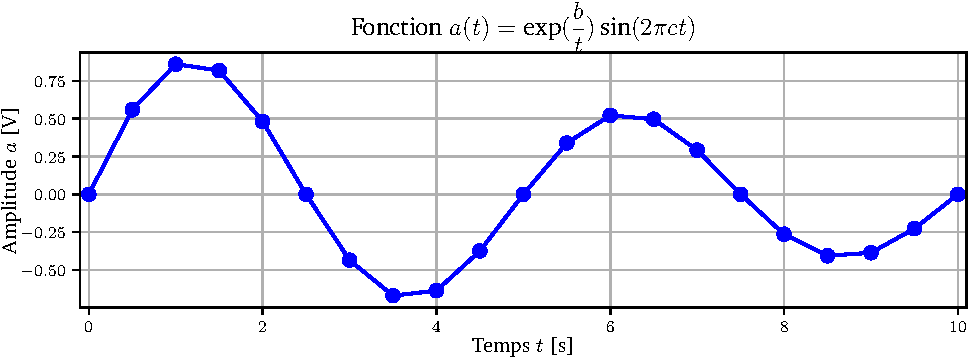
\includegraphics[width = \textwidth]{data/fig_python}}
    \caption{La grande figure.}
  \end{center}
\end{figure*}

% VERSION UNE COLONNE
\begin{figure} % Le * implique si il y a des colonnes,  la figure occupe quand mm toute la largeur.
  \begin{center}
    \frame{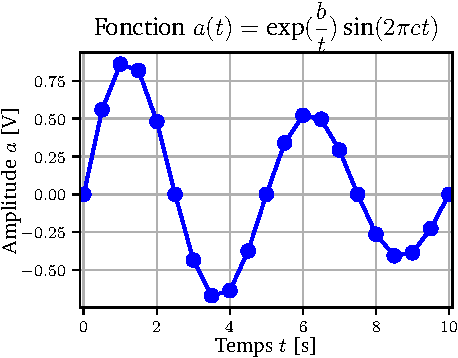
\includegraphics[width = \columnwidth]{data/fig_python_small}}
    \caption{La petite figure.}
  \end{center}
\end{figure}

\blindtext[10]

\end{document}